% LTeX: language=en

\documentclass[a4paper,english]{article}

\usepackage{xcharter-otf}
\usepackage[left=4cm]{geometry}
\usepackage{xspace}
\usepackage[svgnames]{xcolor}
\usepackage{multicol}
\usepackage{hologo}
\usepackage{listings}
\usepackage{showexpl} % examples
\usepackage{mflogo}
\usepackage{babel}
\usepackage{tikz}
\usepackage{url}
\usepackage{tikz}
\usepackage{luamplib}
\usepackage{siunitx}
\usepackage{accsupp}
\usepackage{pdflscape}
\usepackage{fancyvrb,xparse,xargs}
\usepackage[colorlinks]{hyperref}
\setmonofont{FiraCode-Regular}[
BoldFont=FiraCode-Bold,
Contextuals=Alternate, % Activate the calt feature
Scale=MatchLowercase
]
\usepackage{biblatex}
\usepackage{imakeidx}
\makeindex[title=Index, columns=2]
\usepackage[verbatim]{lstfiracode} % Activate ligatures in verbatim
\usepackage[most]{tcolorbox}
\tcbuselibrary{listings,breakable}
\addbibresource{ctan.bib}
\newcommand\package[1]{\href{https://ctan.org/pkg/#1}{#1}}
\newcommand{\ctan}{\textsc{ctan}}
\newtcolorbox{colourband}[1][]{%
arc=0pt,outer arc=0pt,enhanced, breakable, spread sidewards, left*=0pt, right*=0pt, boxrule=0pt, colback=LightSteelBlue!10, #1}


\definecolor{hellgelb}{rgb}{1,1,0.85}
\definecolor{colKeys}{rgb}{0,0,1}
\definecolor{colIdentifier}{rgb}{0,0,0}
\definecolor{colComments}{rgb}{0.3,0.7,0.3}
\definecolor{colString}{rgb}{0,0.5,0}
\definecolor{mpcode}{rgb}{0.5,0.1,0.1}

\lstset{%
  language=metapost,%
  float=hbp,%
  basicstyle=\ttfamily, %
  identifierstyle=\color{DarkSlateGrey}, %
  keywordstyle=\color{DarkBlue}\itshape, %
  stringstyle=\color{Green}, %
  commentstyle=\color{LightSlateGrey}\itshape, %
  columns=flexible, %
  tabsize=4, %
  extendedchars=true, %
  showspaces=false, %
  showstringspaces=false, %
  numbers=left,
  numbersep=1em,
  numberstyle=\tiny\color{gray}, %
  breaklines=true, %
  breakautoindent=true,
  captionpos=b,
  xleftmargin=0em,
  sensitive=true,
  morekeywords=[10]{},
  keywordstyle=[10]\color{Salmon},
  morekeywords=[7]{draw_axis, 
  draw_grad, 
  draw_legends, 
  draw_line, 
  set_axis_color, 
  set_axis_legends, 
  set_kiviat_unit, 
  set_lattice_color, 
  set_lattice_grid,  set_line_mark, 
  set_line_mark_scale, 
  set_line_mark_type, 
  filldraw_line, 
  set_axis,},
  keywordstyle=[7]\color{FireBrick},
  morekeywords=[8]{},
  keywordstyle=[8]\color{Sienna},
  morekeywords=[9]{},
  keywordstyle=[9]\color{Olive}
}
\lstset{explpreset={pos=t,wide=false,rframe={},preset=\centering}}
\lstdefinestyle{syntax}{backgroundcolor=\color{blue!15},numbers=none,xleftmargin=0pt,xrightmargin=0pt,
  frame=single}
\lstdefinestyle{code}{backgroundcolor=\color{red!15},%numbers=left,
  xleftmargin=0pt,xrightmargin=0pt,
  frame=single}

\newtcblisting{mpcode}{
  arc=0pt,outer arc=0pt,
  colback=mpcode!3,
  breakable,
  boxsep=0pt,left=2pt,right=2pt,top=0pt,bottom=0pt, bottomtitle =
  3pt, toptitle=3pt,
  boxrule=0pt,bottomrule=0.pt,toprule=0.pt, toprule at break =
  0pt, bottomrule at break = 0pt,
  listing only,boxsep=0pt,listing
  options={breaklines}
}


\newtcblisting{commandshell}{colback=black,colupper=white,colframe=black,
  arc=0pt,
  listing only,boxsep=0pt,listing
  options={style=tcblatex,language=sh},
  every listing line={\BeginAccSupp{ActualText={}}\textcolor{red}{\small\ttfamily\bfseries user \$> }}\EndAccSupp{}}

\makeatletter
\tcbset{%
    listing metapost/.code={%
        \def\tcbuselistingtext@input{\begin{mplibcode}
        background:=(.988,.976,.976); input \jobname.listing;
        \end{mplibcode}}%
    }
}
\makeatother
\newtcblisting[auto counter,]{ExempleMP}[1][]{%
  arc=0pt,outer arc=0pt,
  colback=FireBrick!3,
  colframe=FireBrick,
  breakable,fontupper=\small,
  boxsep=0pt,left=2pt,right=2pt,top=0pt,bottom=2pt, bottomtitle =
  3pt, toptitle=3pt, lefttitle=5pt,
  boxrule=0pt,bottomrule=0.5pt,toprule=0.5pt, toprule at break =
  0pt, bottomrule at break = 0pt,
  listing side text,
  listing metapost,
  title={\bfseries\sffamily Exemple~\thetcbcounter},
  listing options={breaklines},#1
}


\newcommand\mpkiviat{\texttt{mpkiviat}\xspace}
\newcommand\fichier[1]{\texttt{#1}}
\newcommand\variableGDD[1]{\texttt{\color{Sienna}#1}}
\newcommand\typeMP[1]{\texttt{\color{Tomato}#1}}
\newcommand\typeGDD[1]{\texttt{\color{Sienna}#1}}
\newcommand\foncGDD[1]{\texttt{\color{Sienna}#1}}

\newenvironment{Note}{
  \noindent\textbf{Note~---~}}
  {}



% 
\colorlet{code}{blue!80!black}
\newcommand\cmd{\texttt}
\newcommand\code[1]{\texorpdfstring{\texttt{\color{code}#1}}{#1}}
\newcommand*\cs[1]{\code{\textbackslash #1}}
\newcommand*\macro{\par\bigskip\noindent\hspace{-30pt}%
    \SaveVerb[aftersave={%
     \UseVerb{Vitem}%
    }%
    ]{Vitem}%
 %   \bigskip
}
\newcommand\vitem[1][]{\SaveVerb[%
    aftersave={\item[\textnormal{\UseVerb[#1]{vsave}}]}]{vsave}}
\newcommand*\textme[1]{\textcolor{black}{\rmfamily\textit{#1}}}
\newcommand*\meta[1]{% % meta
  \textme{\ensuremath{\langle}#1\ensuremath{\rangle}}%
}
\newcommand*\optstar{% % optional star
  \meta{\ensuremath{*}}\xspace
}
\DefineShortVerb{\|}
\setlength{\fboxsep}{2pt}
\fvset{%
    codes={\catcode`\«\active \catcode`\×\active },
    defineactive={\makefancyog\makefancytimes},
    formatcom=\color{FireBrick},
    frame=single
}
% rendre «...» équivalent à \meta{...}
{\catcode`\«\active
  \newcommandx\makefancyog[0][addprefix=\global]{%
    \def«##1»{\meta{##1}}}}
% rendre × équivalent à \optstar
{\catcode`\×\active
  \newcommandx\makefancytimes[0][addprefix=\global]{%
    \def×{\optstar{}}}}
 
\NewDocumentEnvironment{Macro}{ov}{%
\Verb+#2+
}{%
}
\newcommand{\return}[1]{~$\rightarrow$~#1}
\newcommand{\indication}[1]{\hfill(\itshape #1)}

\newcommand{\R}{\mathbf{R}}

\begin{document}
%% === Page de garde ===================================================
\thispagestyle{empty}
\begin{tikzpicture}[remember picture, overlay]
 \node[below right, shift={(-4pt,4pt)}] at (current page.north west) {%
   
\includegraphics{fond.pdf}%
 };
\end{tikzpicture}%

\noindent
{\Huge \bfseries \mpkiviat}\\
{\large Package \MP{} to draw Kiviat diagrams}\\[1cm]
\parbox{0.6\textwidth}{
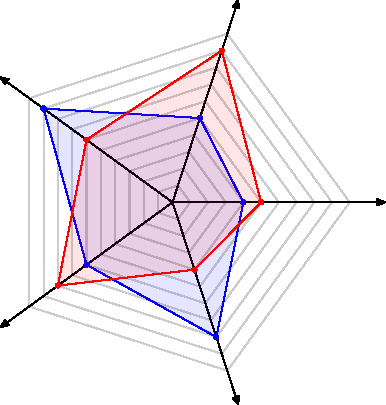
\includegraphics[scale=0.86]{test-2.pdf}
}\hfill
\parbox{0.4\textwidth}{\Large\raggedleft
   \textbf{Contributors}\\
   Maxime \textsc{Chupin}\\
   \url{notezik@gmail.com}
}
\vfill
\begin{center}
Version 0.1, 22th of may 2024\\
\url{https://gitlab.gutenberg-asso.fr/mchupin/mpkiviat}
\end{center}
%% == Page de garde ====================================================
\newpage

\begin{abstract}
  This \hologo{METAPOST} package allows to draw Kiviat diagram (or radar chart,
  web chart, spider chart, etc.).
\end{abstract}

\tableofcontents


\section{Introduction}

\mpkiviat is a package to draw Kiviat diagram (web chart, spider chart, spider
graph, spider web chart, star chart, star plot, cobweb chart, irregular polygon,or
polar chart) with \MP~\cite{ctan-metapost}.

\section{Installation}

\mpkiviat is on \ctan{} and can also be installed via the package manager of
your distribution.

\begin{center}
  \url{https://www.ctan.org/pkg/mpkiviat}
\end{center}


\subsection{With \TeX live under Linux or macOS}

To install \mpkiviat with \TeX Live, you will have to create the directory
\lstinline+texmf+  in your \lstinline+home+. 

\begin{commandshell}
mkdir ~/texmf
\end{commandshell}

Then, you will have to place the \lstinline+mpkiviat.mp+ file in 
\begin{center}
  \lstinline+~/texmf/metapost/mpkiviat/+
\end{center}


Once this is done, \mpkiviat will be loaded with the classic \MP{}
input code
\begin{mpcode}
input mpkiviat
\end{mpcode}

\subsection{With Mik\TeX{} and Windows}

These two systems are unknown to the author of \mpkiviat, so we
refer you to the Mik\TeX documentation concerning the addition of local packages:
\begin{center}
  \url{http://docs.miktex.org/manual/localadditions.html}
\end{center}



\subsection{Dependencies}


\mpkiviat depends, of course on \MP~\cite{ctan-metapost}, as well as the
packages and---if \mpkiviat is not used with
\hologo{LuaLaTeX}~\cite{ctan-lualatex-doc,ctan-luatex} and the
\package{luamplib} or \package{minim-mp}~\cite{ctan-luamplib,ctan-minim-mp} 
packages---the \package{latexmp}~\cite{ctan-latexmp} package. 


\section{Axis and lattice}

\begin{colourband}
  \macro|set_axis(«list of axis names»)|
\medskip

  The \meta{list of axis names} is a list delimited by commas with the names of
  the different axis as \typeMP{string} (e.g.
  \lstinline+"Légumes","Fruits","Produits laitiers"+).
  \index{set_axis@\lstinline+set_axis+}
\end{colourband}

The command to draw the Kiviat background is the following:


\begin{colourband}
  \macro|draw_axis|
  \index{draw_axis@\lstinline+draw_axis+}
\end{colourband}

The combinaison of these two commands produces, for example:
\begin{ExempleMP}[sidebyside=false]
input mpkiviat;
beginfig(1);
set_axis("Légumes","Viande","Lait","Pain","Poissons");
draw_axis;
endfig;
\end{ExempleMP}

By default, legend of each axis are written, but you can avoid that using the
following command:

\begin{colourband}
  \macro|set_axis_legends(«boolean»)|
  \medskip 

  \begin{description}
    \item[\meta{boolean}:] \typeMP{true} or \typeMP{false} 
  \end{description}
  \index{set_axis_legends@\lstinline+set_axis_legends+}
\end{colourband}


Default value for each axis is 10, and there is 10 steps for the lattice. You
can redefine that with the following command that \emph{should be set before the
drawing command} :
\begin{colourband}
  \macro|set_lattice_grid(«unit»,«max»)|
\medskip

  \begin{description}
    \item[\meta{unit}:] (\typeMP{numeric}) is the interval between two lines of the lattice;
    \item[\meta{max}:] (\typeMP{numeric}) is the maximum value for each axis.  
  \end{description}
  \index{set_lattice_grid@\lstinline+set_lattice_grid+}
\end{colourband}

You can print the graduations for the lattice with the following command:
\begin{colourband}
  \macro|draw_grad(«prefix»,«suffix»,«axis number»)|
\medskip

\begin{description}
  \item[\meta{prefix}:] (\typeMP{string}) is a string to add before each graduation;
  \item[\meta{suffix}:] (\typeMP{suffix}) is a string to add after each graduation;
  \item[\meta{axis number}:] (\typeMP{numeric}) is an integer to choose the axis
  used for printing the graduations.   
\end{description}
\index{draw_grad@\lstinline+draw_grad+}
\end{colourband}

\mpkiviat defines a unit that can be modified to scale the entire graph with the
following command (that must be used before the command \lstinline+set_axis+).

\begin{colourband}
  \macro|set_kiviat_unit(«unit»)|
\medskip

\begin{description}
  \item[\meta{unit}:] (\typeMP{string}, default \SI{0.3}{cm}) is the unit to
  draw the graph.   
\end{description}
\index{set_kiviat_unit@\lstinline+set_kiviat_unit+}
\end{colourband}

One can set colors for the axis and the lattice with the two following commands. 


\begin{colourband}
  \macro|set_axis_color(«color»)|
\medskip

  \begin{description}
    \item[\meta{color}:] (\typeMP{color}) is the color for drawing the axis arrows.  
  \end{description}
  \index{set_axis_color@\lstinline+set_axis_color+}
\end{colourband}


\begin{colourband}
  \macro|set_lattice_color(«color»)|
\medskip

  \begin{description}
    \item[\meta{color}:] (\typeMP{color}) is the color for drawing the lattice.  
  \end{description}
  \index{set_lattice_color@\lstinline+set_lattice_color+}
\end{colourband}



The following example illustrates some of the previous commands. 

\begin{ExempleMP}[sidebyside=false]
input mpkiviat;
beginfig(1);
set_kiviat_unit(0.4cm);
set_axis("Légumes","Viande","Lait","Pain","Poissons");
set_axis_color((0.7,0.1,0.1));
set_lattice_color((0.5,0.5,0.9));
set_lattice_grid(100,600);
draw_axis;
draw_grad("","~€",3);
endfig;
\end{ExempleMP}


\section{Add lines}

Once you have drawn the background, you can add lines for your Kiviat diagram. 
The basic command to do that is the following:

\begin{colourband}
  \macro|draw_line(«list of values»)(«color»)|
\medskip

  \begin{description}
    \item[\meta{list of value}:] (list of \typeMP{string}) values for the
    different axis of the Kiviat diagram (e.g. \lstinline+"9","2","3"+). The
    values must match the settings of the lattice. 
    \item[\meta{color}:] (\typeMP{color}) is the color for drawing the line.  
  \end{description}
  \index{draw_line@\lstinline+draw_line+}
\end{colourband}

You can also draw and fill a Kiviat line with the following command:

\begin{colourband}
  \macro|filldraw_line(«list of values»)(«color»)|
\medskip

  \begin{description}
    \item[\meta{list of value}:] (list of \typeMP{string}) values for the
    different axis of the Kiviat diagram (e.g. \lstinline+"9","2","3"+). The
    values must match the settings of the lattice. 
    \item[\meta{color}:] (\typeMP{color}) is the color for drawing the line. The
    filling color is transparent\footnote{Thanks to Anthony Phan \MP{} code : \url{http://www-math.univ-poitiers.fr/~phan/metalpha.html}.}
  \end{description}
  \index{filldraw_line@\lstinline+filldraw_line+}
\end{colourband}

By default, there is mark on a Kiviat line. You can remove marks with the
following command, setting the booelan argument to \lstinline+false+. 



\begin{colourband}
  \macro|set_line_mark(«boolean»)|
\medskip


\begin{description}
  \item[\meta{boolean}:] \typeMP{true} or \typeMP{false} 
\end{description}
  \index{set_line_mark@\lstinline+set_line_mark+}
\end{colourband}

You can also choose the type of mark. \mpkiviat provides three types :
\lstinline+"square"+, by default, \lstinline+"circle"+ and \lstinline+"custom"+.
To choose one of them, you have to use the following command: 
\begin{colourband}
  \macro|set_line_mark_type(«type»)|
\medskip


\begin{description}
  \item[\meta{type}:] (\typeMP{string})  \lstinline+"square"+, by default,
  \lstinline+"circle"+ and \lstinline+"custom"+. 
\end{description}
  \index{set_line_mark_type@\lstinline+set_line_mark_type+}
\end{colourband}

If you choose \lstinline+custom+, you will have to define a macro
\lstinline+line_mark_custom+ that take a \typeMP{pair} as argument and that
define a cycled path shifted around the \typeMP{pair}. For instance, the
\lstinline+line_mark_square+ command is defined as:
\begin{mpcode}
def line_mark_square(expr p)=
  (((-1,-1)--(1,-1)--(1,1)--(-1,1)--cycle scaled _line_mark_scale) shifted p)
enddef;
\end{mpcode}

You can adjust the size of the marks using the following scaling macro:
\begin{colourband}
  \macro|set_line_mark_scale(«scaling factor»)|
\medskip


\begin{description}
  \item[\meta{scaling factor}:] is a \typeMP{numeric} that is, by default, 1. 
\end{description}
  \index{set_line_mark_scale@\lstinline+set_line_mark_scale+}
\end{colourband}

Here is an example that illustrates some of the previous commands. 

\begin{ExempleMP}[sidebyside=false]
input mpkiviat;
beginfig(1);
set_lattice_grid(100,500);
set_kiviat_unit(0.4cm);
set_axis("McCabe","LOC","Live Variables","Halstead N","Variablenspanne");
draw_axis;

filldraw_line(400,300,380,200,250)(red);
set_line_mark_type("circle");
filldraw_line(300,320,180,400,150)(blue);
set_line_mark_type("square");
set_line_mark_scale(2);
filldraw_line(100,420,280,200,50)(green);
endfig;
\end{ExempleMP}

\section{Legends}

\mpkiviat provides the following command to add legends to a Kiviat diagram:

\begin{colourband}
  \macro|draw_legends.«place»(«list of names»)|
\medskip


\begin{description}
  \item[\meta{place}:] is one of the standard \MP{} suffixes :
  empty, \lstinline+lft+, \lstinline+rt+, \lstinline+top+,
  \lstinline+bot+, \lstinline+ulft+, \lstinline+urt+, \lstinline+llft+ and
  \lstinline+lrt+. The legend is placed at the given place of the bounding box
  of the complete Kiviat diagram (without the legend). If it is empty, the
  default place is \lstinline+rt+. 
  \item[\meta{list of names}:] is the list of \typeMP{string} of names for the
  different lines in the order of the construction.   
\end{description}
  \index{draw_legends@\lstinline+draw_legends+}
\end{colourband}

\begin{ExempleMP}[sidebyside=false]
input mpkiviat;
beginfig(1);
set_lattice_grid(100,500);
set_kiviat_unit(0.4cm);
set_axis("McCabe","LOC","Live Variables","Halstead N","Variablenspanne");
draw_axis;

filldraw_line(400,300,380,200,250)(red);
set_line_mark_type("circle");
filldraw_line(300,320,180,400,150)(blue);
set_line_mark_type("square");
set_line_mark_scale(2);
filldraw_line(100,420,280,200,50)(green);
draw_legends.lrt("Première", "Deuxième", "Troisième");
endfig;
\end{ExempleMP}

\printbibliography
\printindex

\end{document}
